\chapter{Experiments}

\todo{for motivation, maybe consider the introduction \href{https://arxiv.org/pdf/1712.03346.pdf}{here}}

In this chapter, we report on the experiments within protein machine learning that we have performed.

In section \ref{sec:variational_autoencoders_experiement}, we explore the usefulness of the variational autoencoder on protein sequences. Specifically, we train a variational autoencoder model on sequences within single protein families, obtaining a seperate model for each family. The variational autoencoder does not handle variable-length sequences though, so each family of proteins must be aligned to a single length.

In section \ref{sec:unirep_experiment}, we turn to a model with a significantly different approach to the protein machine learning problem, the UniRep model \cite{alley2019unified}. UniRep is a recurrent model, and can thus handle variable-length sequences, and can thus be trained on global protein databases. We explore the performance of a variant of the UniRep model on downstream tasks.

\section{General Methodology}
For all of our experiments, we utilized PyTorch \cite{NEURIPS2019_9015}, a modern machine learning framework. We preferred PyTorch over the alternatives due to its flexible yet concise usage. We also had good experiences using it in past projects.

\section{Variational Autoencoders on Aligned Protein Families}
\label{sec:variational_autoencoders_experiement}

As previously discussed \todo{make sure this is actually discussed}, producing global representations, meant to be utilized for the entire space of all proteins, may be too optimistic and performance may suffer in the local protein family landscapes. A model that only tries to capture representations of a single protein family may be more feasible, because the space of possibilities and variance in the sequences are vastly reduced. Training a model on such a smaller data-set is also much simpler, requiring less memory and less time before convergence.

With this in mind, we decided to try out models that work on single protein families first. There are more benefits to only working with a single protein family -- it is possible to align the sequences to a single predetermined length. The alignment to a single length allows simple densely connected neural networks to work very effectively on the proteins, since the absoluteness of the sequence positions makes it easy for the weights in the densely connected layers to adjust for each position.

It just so happens that the archetypical variational autoencoder (VAE) uses densely connected neural networks for its encoder and decoder architecture. Also, VAEs have previously been shown to be effective on aligned protein sequence families \cite{riesselman2018deep}. Thus we had good reason to believe that this would be a fruitful experiment.

We constructed a VAE model based on PyTorch's own VAE example\footnote{\url{https://github.com/pytorch/examples/blob/master/vae/main.py}}. We then modified this model, to utilize some of the ideas from \cite{riesselman2018deep}.

For example, we added weights on each sequence, in order to reduce human sampling bias and evolutionary bias. These weights are multiplied on the loss for the sequences, and in that way influences how the model weights each sequence in its optimization. Each sequence's weight is calculated as the reciprocal of the number of neighbours the sequence has, where "neighbour" means a sequence within 0.2 Hamming distance.

Another significant deviation from a standard VAE is the addition of Bayesian weights on the linear layers of the decoder. Rather than the decoder using standard deterministic linear layers, it uses probabilistic linear layers. Rather than having a single deterministic weight and bias, the model samples a weight and bias for the layers every time they are used\footnote{For performance reasons, the model actually samples a single weight and bias for an entire batch.}. This means that the model optimizes not just a singular linear layer -- instead, it optimizes a distribution of linear layers.

This distribution of layers is particularly useful at evaluation time. By running the model multiple times on the evaluation data, the model samples different linear layers every time. Effectively, this constructs an ensemble of models of an unlimited size, because the distribution is continuous. Ensembles of models are known to, in general, perform better than single models in isolation. The intuition behind this, is that different models can compensate for each others' weaknesses and shortcomings, thus providing a model that performs better than the mean of the individual models' performances.

We trained one model for each protein family we examined, but kept the architecture of the model constant throughout. The training process uses both the encoder and the decoder. The encoder compressed the sequence from its original size (that is, a flattened one-hot encoding) into two 1500-dimensional layers, before reaching the 30-dimensional probabilistic bottleneck representation. Samples are drawn from the representation, which are sent into the decoder, which has a 100-dimensional layer, followed by a 2000-dimensional layer, before reaching the original sequence size again.

For data, we use the sequence alignments made available by \cite{riesselman2018deep}. We train each model on 80\% of the aligned sequences, using the rest for validation, with 128 batch size. We continue training until we see no improvement on the validation score for 50 epochs, and keep the model that performed best on the validation set. This leads to a total training of a few hundred epochs, or under an hour of training on the NVIDIA Titan X GPUs we used.

\subsection{Results}
When evaluating the model, we are primarily interested in the usefulness of the representations produced by the encoder. Thus, the decoder is only used for training the encoder, or for recovering the protein sequence from the representation given by the encoder. We evaluate the representation by examining its properties, as well as using it for a predictive downstream task.

Figure \ref{fig:2dimvae} shows the mean of the representations of proteins from the $\beta$-lactamase protein family, colored by phylum, as produced by a VAE model of the same dimension as described earlier, except with a 2-dimensional bottleneck size, so that we can plot the representation. The structure of the representations resemble that of a phylogenetic tree, suggesting that the model correctly identifies the evolutionary similarities between the different variants of $\beta$-lactamase. A similar phylogenetic tree-like structure is seen when using the model on other protein families.

\begin{figure}[ht]
    \centering
    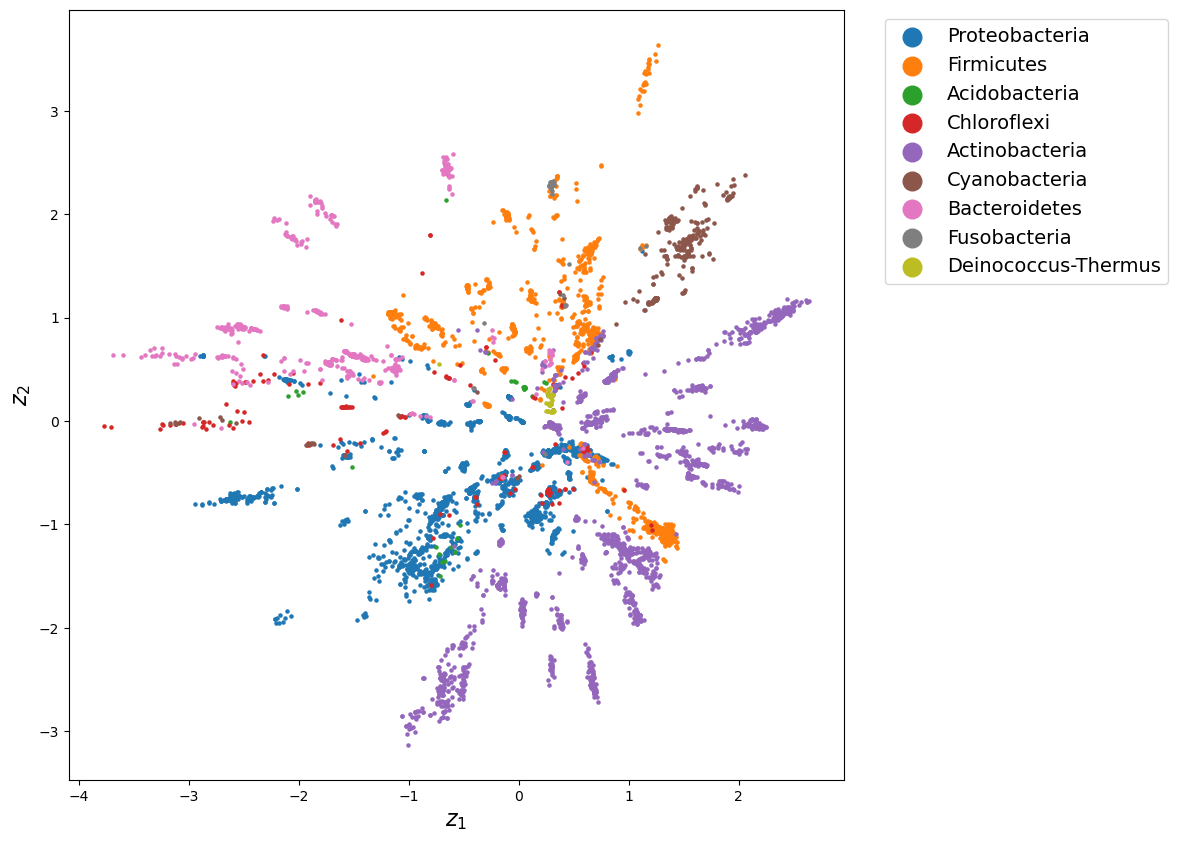
\includegraphics[width = \linewidth]{report/figures/vae_representation2d.png}
    \caption{Mean of the protein representations of selected phylums of $\beta$-lactamase, produced by a VAE model with a bottleneck layer size of 2.}
    \label{fig:2dimvae}
\end{figure}

\section{UniRep: A Recurrent Global Model}
\label{sec:unirep_experiment}
The variational autoencoder described above fills the role of a local protein model. In order to compare the performance of global and local protein models, we require a model capable of training on global protein data. The UniRep model fills this purpose.

UniRep was proposed in 2019 \cite{alley2019unified}, and utilizes a recurrent neural network (RNN) to encode proteins into a single representation vector of a set dimensionality. Because it uses an RNN, it is capable of handling the variable lengths of proteins without needing an alignment. This makes it able to work on global protein space, leading to what the authors of UniRep refers to as a ``unified representation'' -- hence the name.

The canonical UniRep model presented in \cite{alley2019unified} uses an mLSTM (multiplicative  variant of the common LSTM RNN) with a hidden state size of 1900, as the RNN inside the model. Additionally, it utilizes truncated backpropogation during training.

We have previously (\todo{cite UniRep project, somehow}) worked with UniRep and explored the significance of the above hyperparameters. We found that the choice of RNN among mLSTM, LSTM or GRU is not significant, and that smaller hidden state sizes can achieve nearly equivalent performance. The choice of RNN and hidden state size can however have a major impact on the computational performance of the model. We found that truncated backpropogation only made the model perform marginally worse. 

In accordance with the above, we decided not to use the canonical UniRep model, and instead opted to use an LSTM with a 512 hidden state size, without truncated backpropogation. Our previous experiments suggests that the difference between the canonical UniRep model and this variant should not be significant. At the same time, our model is smaller and can make use of PyTorch's inbuilt LSTM module, both of which contribute to a much more computationally cheap model.


